%%%%%%%%%%%%%%%%%%%%%%%%%%%%%%%%%%%%%%%%%%%%%%%%%%%%%%%%%%%%%%%%%%%%%%%%%%%%%%%%%%%%%%%%%
% Autor:        Aguilar Enriquez, Paul Sebastian a.k.a. Penserbjorne
% Fecha:        05/02/2017
% Descripción:  Plantilla base para actividades o tareas.
%%%%%%%%%%%%%%%%%%%%%%%%%%%%%%%%%%%%%%%%%%%%%%%%%%%%%%%%%%%%%%%%%%%%%%%%%%%%%%%%%%%%%%%%%

\documentclass[a4paper,11pt]{article}                 % Papel tamaño carta, texto de 11pt.

\usepackage[top=2cm, bottom=2cm, left=2.2cm, right=2.2cm]{geometry} % Margenes
\usepackage[T1]{fontenc}                              % Indicamos la codificacion de las fuentes.
\usepackage[utf8x]{inputenc}                          % Definimos la codificacion.
\usepackage{lmodern}                                  % Para poder usar acentos.
\usepackage[spanish,es-nodecimaldot]{babel}           % Usaremos idioma español y punto decimal.
\usepackage{amsmath}                                  % Para formulas matematicas.
\usepackage{graphicx}                                 % Para imagenes.
\usepackage{float}                                    % Para posicionar objetos.
\usepackage{booktabs}                                 % Para formatear tablas.
\usepackage{hyperref}                                 % Para enlaces y referencias.
\usepackage{listings}                                 % Para código
\usepackage[numbered,framed]{matlab-prettifier}       % Para código M

%%%%%%%%%%%%%%%%%%%%%%%%%%%%%%%%%%%%%%%%%%%%%%%%%%%%%%%%%%%%%%%%%%%%%%%%%%%%%%%%%%%%%%%%%

% Los logos tienen posiciones relativas al nombre de la escuela.
% Cada imagen esta desplazada con respecto al texto, en este caso nombre de la univseridad.
% No se necesitan paquetes adicionales, el entorno estandar para imagenes de LaTeX puede hacerlo.
% El truco esta en definir una imagen de tamaño cero, asi no afecta al centrar los titulos.
\def\logoUNAM{%
  \begin{picture}(0,0)\unitlength=1cm
    \put (-3.5,-3) {
\includegraphics[width=8em]{../images/escudo-unam}}
  \end{picture}
}

\def\logoFI{%
  \begin{picture}(0,0)\unitlength=1cm
    \put (0.5,-3) {
\includegraphics[width=8em]{../images/escudo-fi}}
  \end{picture}
}

%%%%%%%%%%%%%%%%%%%%%%%%%%%%%%%%%%%%%%%%%%%%%%%%%%%%%%%%%%%%%%%%%%%%%%%%%%%%%%%%%%%%%%%%%

\author{Aguilar Enriquez, Paul Sebastian --- 415028130}  % Autor de la actividad.
\title{Práctica 01}                % Titulo de la actividad.
\date{26/08/2019}                                           % Fecha de entrega.
\def\universidad{Universidad Nacional Autónoma de México}   % Nombre de la universidad.
\def\facultad{Facultad de Ingeniería}                              % Nombre de la facultdad.
\def\semestre{2020-1}                                     % Semestre lectivo.
\def\materia{Temas selectos de sistemas inteligentes - Grupo 2}               % Nombre de la materia y grupo.
\makeatletter

%%%%%%%%%%%%%%%%%%%%%%%%%%%%%%%%%%%%%%%%%%%%%%%%%%%%%%%%%%%%%%%%%%%%%%%%%%%%%%%%%%%%%%%%%

\begin{document}
  
  % Titulo del documento con logos.
  \begin{center}
    \logoUNAM {\Large \universidad} \logoFI\par
    {\large \facultad}\par
    \semestre\par
    \materia\par
    \@author\par
    \@date\par
    \@title
  \end{center}

  \hrulefill\par

  \pagenumbering{gobble}                              % Oculta el numero de pagina.
%  \tableofcontents                                    % Crea el indice o tabla de contenido.

%%%%%%%%%%%%%%%%%%%%%%%%%%%%%%%%%%%%%%%%%%%%%%%%%%%%%%%%%%%%%%%%%%%%%%%%%%%%%%%%%%%%%%%%%

  %\newpage                                            % Inserta una pagina nueva.
  \pagenumbering{arabic}                              % Muestra el numero de pagina.
  
  \section{Código fuente}
  
  \lstinputlisting[language=Matlab]{practica01.m}
  
  \newpage                                            % Inserta una pagina nueva.
  \section{Salida del script}
  
    \lstinputlisting[language=Matlab]{practica01.m.out}
  
  \newpage                                            % Inserta una pagina nueva.
  \section{Gráficas}
  
  \begin{figure}[H]
    \begin{center}
      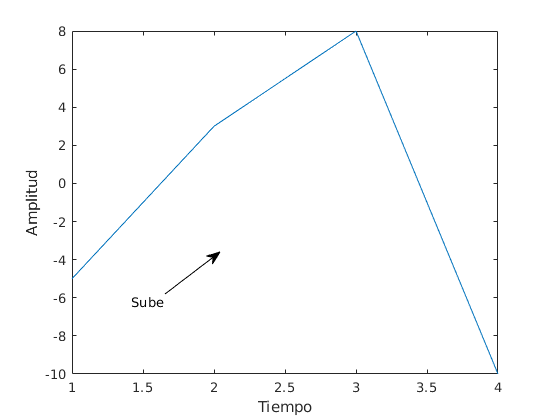
\includegraphics[height=10cm]{ejercicio01.png}
      \caption{Figura del ejercicio 01}
      \label{fig:01}
    \end{center}
  \end{figure}

  \begin{figure}[H]
    \begin{center}
      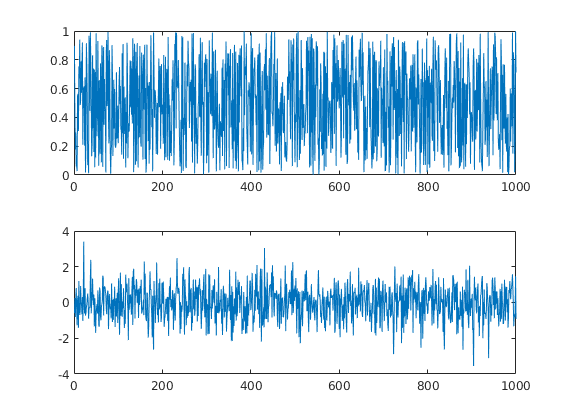
\includegraphics[height=10cm]{ejercicio02.png}
      \caption{Figura del ejercicio 02}
      \label{fig:02}
    \end{center}
  \end{figure}
  
  
%%%%%%%%%%%%%%%%%%%%%%%%%%%%%%%%%%%%%%%%%%%%%%%%%%%%%%%%%%%%%%%%%%%%%%%%%%%%%%%%%%%%%%%%%

\end{document}
